\section{DAPHNE test results}
\subsection{DAPHNE: cold and warm electronics interface}

The DAPHNE board is the warm electronics interface with the cold electronics that will operate outside the criostat. DAPHNE provides power to both amplifier and SiPMs, re-amplifies and digitizes the signals from the PD modules, formats and transmits the generated data to the DAQ system of the experiment. 

\begin{figure}[h]
\centering
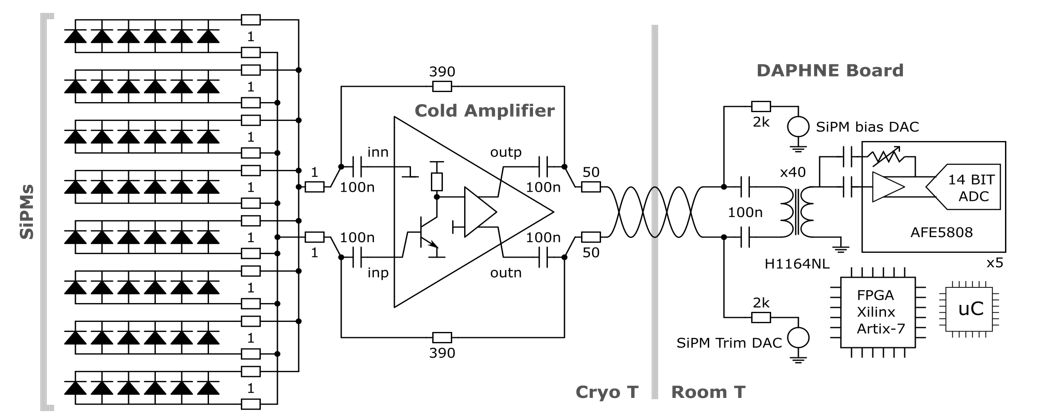
\includegraphics[width=100mm]{Images/pd_electronics.png}
\caption[]{Schematic of the PD cold and warm electronics.}
\label{fig:pd_electronics}
\end{figure}

At Milano-Bicocca, our main focus with the DAPHNE development is the interface between DAPHNE's analog front end (AFE), the Texas Intruments AFE5808 and the cold electronics, to achieve the best possible signal fidelity, SNR, demonstrate the capability to trigger on single P.E. signal and to control precisely the trigger level in each channel.

In the following subsections, various test that were instrumental to advance towards the demostration that the PD electronics system can comply with the DUNE's experiment requirements. 

\subsection{Dynamic range and signal fidelity}

The dynamic range requirement for the PD system is 2000 photoelectrons. According to the simulation and measured data, a single P.E. can be considered to have a peak to peak value of around 400 ${\mu}V$ for 45\% PDE at the input of DAPHNE's AFE. The AFE5808 \cite{afe5808a} can safely be configured to have a linear response for an input signal up to $1Vpp$. Considering that 2000 P.E. is around 800 $mVpp$, the AFE5808 should handle the required dynamic range with a 20\% safety margin. There is although a drawback, the AFE5808 has no configurable OFFSET for the first stage low-noise amplifier (LNA) reference voltage and since the SiPMs signals are in escence unipolar signals, only half of the dynamic range can be exploited. To address this issue, DAPHNE designers had to implement an external OFFSET correction circuit to modify the reference voltage at the input of the LNA to allow the full dynamic range to be exploited.

\begin{figure}[h]
\centering
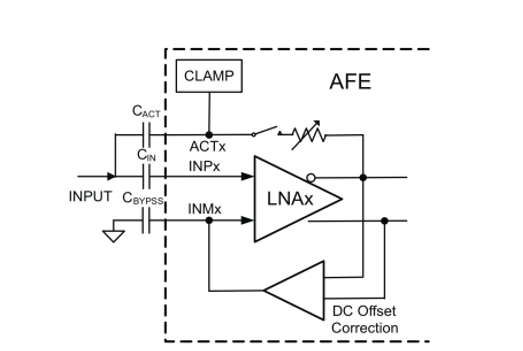
\includegraphics[width=100mm]{Images/AFE5808_frontend.png}
\caption[]{Schematic the AFE5808 input LNA, active termination and DC offset correction. \cite{afe5808a}}
\label{fig:afe_frontend}
\end{figure}

Figure \ref{fig:afe_frontend} shows the input LNA. The signal arrives from the cold amplifier via twisted pair and passes throught a 1:1 balun transformer to perform the differential to single ended convertion and finally gets terminated by the AFE5808's active termination circuit $ACTx$. The active termination is user configurable, but in order to match the system impedance, 100$\Omega$ termination must be selected. The OFFSET correction circuit is not shown but is simple in nature, it consist in a DAC (Digital to Analog Converter) connected to the $INPx$ pin via a 20 $k\Omega$ resistor, making a voltage divider with the internal pull-up resistor and voltage reference.

\begin{figure}[h]
\centering
\subfigure[]{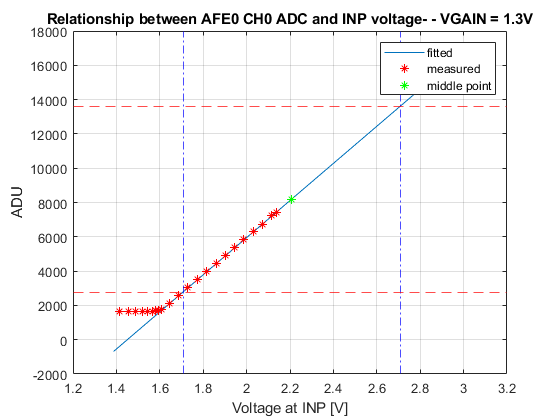
\includegraphics[width=60mm]{Images/linear_vgain_13.png}}
\subfigure[]{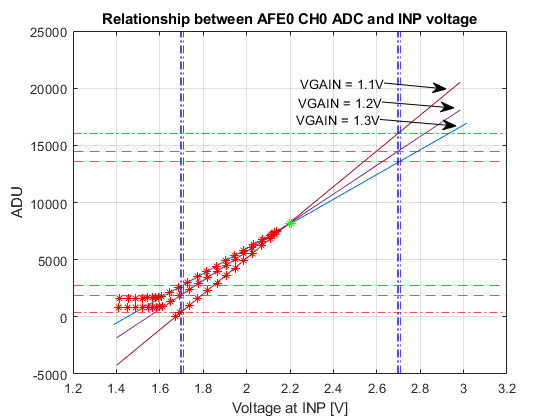
\includegraphics[width=60mm]{Images/linear_vgain_all.png}}
\caption[]{Linearity response of the AFE5808 and the OFFSET circuit. a) Attenuation: VGAIN 1.3V. b) Attenuation: VGAIN 1.1V - 1.2V - 1.3V.  }
\label{fig:offset_test}
\end{figure}

Figure \ref{fig:offset_test} shows the response of the AFE5808 when the OFFSET circuit is set to a specific value. Both figures \ref{fig:offset_test}a and \ref{fig:offset_test}b show the relatioship between the measured voltage at $INPx$ and the average $ADU$ (Analog Digital Unit) acquired by DAPHNE in channel 0. The vertical blue lines indicate the limits of the linear input of $1Vpp$, and the horizontal red lines are the intersection of the blue lines with the fitted line of the measured data, which indicate the expected linear region in $ADU$ units. The green asterisk indicate the midpoint OFFSET where the maximun voltage swing can be obtained for a sinusoidal voltage input. Note that for high attenuation configurations, the AFE5808 clamp effect can be noted at low ADU values but there is still a small linear region below $1Vpp$ (horizontal red lines) guaranteed linear zone. The effect of decreasing the attenuation can be seen in figure \ref{fig:offset_test}b, where the AFE5808 can be configured to have full linear range for $2^{14}$ ADU, as is for the case of $VGAIN = 1.1V$ (VGAIN is the programmable attenuator voltage control) where the clamping effect is below and above the ADU range giving a straight line for every voltage range at $INP$. This relationship estimates the overall gain of each AFE5808 channel at specific configuration, and has units of $\frac{ADU}{V}$. 

The signal fidelity of the acquired waveforms was a concern, specially the effect of the OFFSET correction circuit could have in the internal amplification and digitization processes of the AFE5808. A sinusoidal signal with a 200 $mVpp$ is injected at the input and waveforms are acquired stepping OFFSET values. Figure \ref{fig:fidelity_1} shows the acquired sinusoidal waveform at the top. The bottom waveforms were acquired with an oscilloscope probing the $INP$ node of the AFE5808 channel that is under test. As can bee seen in figure \ref{fig:fidelity_1}a, both waveforms present a clipping effect that distorts the signal. According to what was presented above, this clipping effect should not occur at this point and moreover, it's occurring at the opposite semicycle as the ADU OFFSET moves towards 0. 

\begin{figure}[h]
\centering
\subfigure[]{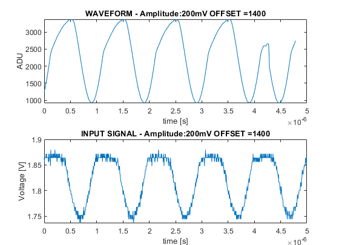
\includegraphics[width=60mm]{Images/fidelity_200.png}}
\subfigure[]{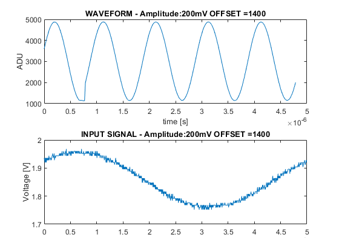
\includegraphics[width=60mm]{Images/fidelity_200_corrected.png}}
\caption[]{Acquired waveforms when a sinusoidal signal is injected at the input of the AFE5808. a) 100 $\Omega$ active termination ON . b) Active termination OFF (passive $100 \Omega$ termination) }
\label{fig:fidelity_1}
\end{figure}

It was noted that the active termination circuit $ACTx$, shown in figure \ref{fig:afe_frontend}, has a clamp feature. After deliberation, it was concluded that the clipping issue may have the following explanation: As the $INP$ value decreases due to the effect of the OFFSET correction, the inverted DC output value of the LNA increases moving closer to the CLAMP activation value. The CLAMP can be removed by deactivating the $ACTx$ circuit, breaking the feedback loop. At this point, a physical $100\Omega$ resistor had to be added in order to correctly terminate the line. Figure \ref{fig:fidelity_1}b shows the result of these modifications, where both acquired and probed signals no longer suffer from the clipping effect. 

\begin{figure}[h]
\centering
\subfigure[]{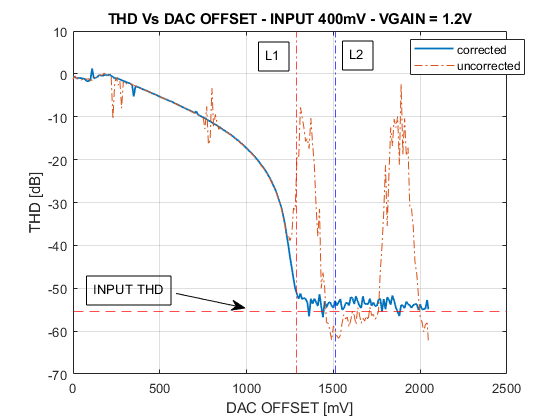
\includegraphics[width=60mm]{Images/thd_1.png}}
\subfigure[]{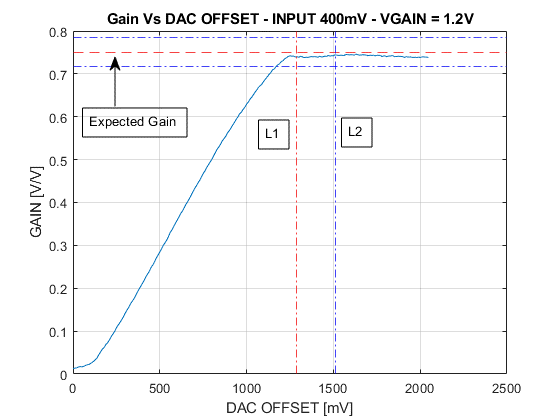
\includegraphics[width=60mm]{Images/gain_1.png}}
\caption[]{Total harmonic distortion (THD) and GAIN of the acquired signal for stepping values of OFFSET configuration.  a) THD b) GAIN }
\label{fig:thd_gain}
\end{figure}

Having solved the aforementioned issue and in order to quantify the fidelity of the acquisition with respect of the OFFSET configuration, measurements of the total harmonic distortion and signal gain were performed with stepping OFFSET configurations. Figure \ref{fig:thd_gain}a shows the THD figures for different OFFSET configurations. A $400 mVpp$ sinusoidal signal was injected and probed at the input. The input THD from the probed signal was calculated and serves as a reference (red dashed line) for the THD calculations of the acquired waveforms. The figure can be explained as follows: As the OFFSET value increases towards the midpoint, the THD figures should improve towards the limit of the reference THD value. The limit at which the acquired THD reaches the reference can be estimated using the data from figure \ref{fig:offset_test}b, denoted $L1$ and $L2$, marks the beginning of the OFFSET linear regions. Figure \ref{fig:thd_gain}b shows the gain for stepping OFFSET values where the expected gain can also be estimated from the referred data in figure \ref{fig:offset_test}b. For both figures \ref{fig:thd_gain}a and \ref{fig:thd_gain}b, the measured THD and gain values approximates to the expected values in the expected linear region, therefore, it is concluded that the OFFSET correction circuit does not have a degrading effect in the signal fidelity of the acquired waveforms.  

\subsection{Noise issues in the DAPHNE board}

In the previous subsection, an effort has been made to achieve the best possible signal fidelity and to guarantee that the subsystems around the AFE do not affect the acquisition mechanisms. Large test signals were injected to verify the fidelity and a serious problem was identified and resolved. Moving forward to small signals, in the range of single P.E. waveforms, the main concern is to achieve the lowest noise figures possible to obtain the best SNR. 

The first calibrations tests integrating the cold amplifier with DAPHNE failed. Even at large amplification factors, DAPHNE had very poor SNR performance.  

Figure \ref{fig:noise_1} shows the average frequency spectrum of 10000 waveforms. The yellow plot shows various spurious frequency components peaks, from these, two peaks show larger amplitude, 630 $kHz$ and 1.53 $MHz$. At this point, the DAPHNE board was probed extensively to search and pinpoint the origin of these components. The noise components was found to be injected at the input nodes before the capacitors that decouple the bias and trim circuitry to power the SiPMs, and originate from the DC-DC voltage converters circuitry, where the 48V input voltage gets converted to the numerous voltage rails that DAPHNE subsystems power from, specifically the +5V, -5V analog and SiPM bias voltage rails.

The referred noise from the power rails affected subsystems that were directly connected to the AFEs input and are critical for the PD systems performance and monitoring. These systems are:

\begin{enumerate}
    \item The analog multiplexer for the SiPMs current monitor systems
    \item The BIAS supply circuitry.
    \item the BIAS TRIM voltage circuitry. 
\end{enumerate}

The cited subsystems were found to be vulnerable due to inadequate PSSR (Power Supply Rejection Ratio). Figure \ref{fig:noise_1} also shows spectrum figures when these subsystems are disconnected, confirming that the overall noise gets injected through them via their power supply rails. 

\begin{figure}[h]
\centering
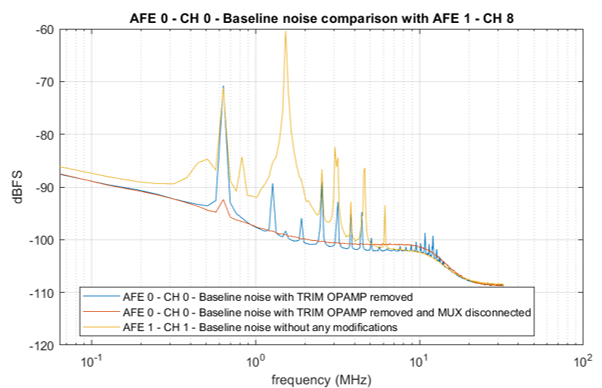
\includegraphics[width=100mm]{Images/noise_1.png}
\caption[]{Average frequency spectrum of acquire signals.}
\label{fig:noise_1}
\end{figure}

The approach taken to solve this problem was to apply filter patches at the output of these subsystems given that it was not possible to apply filters at the source of the noise, the DC-DC converters, without the risk of seriously damaging the boards in the process. Three different patches were applied and each of them with satisfactory results. 

The patch was selected considering the number of extra components and difficulty of implementation. Figure \ref{fig:patches}a show the schematic of the selected filter patch, where an extra capacitor and resistor were inserted after the TRIM node to form a low pass filter. Also, an extra capacitor was inserted between GND and S2 was inserted to filter noise components that are injected through this node. The other patches 1 and 2 are not shown, but they produce the same result with slight variations of patch 3. Other changes that were made are the addition of inductors at the subsystem's power rails to increase the PSSR, and changes to components in the BIAS circuitry to filter better the SiPMs BIAS voltages. Figure \ref{fig:patches}b show the frequency spectrum of the input after the patches are applied to different AFE chips. The overall comparison show similar noise suppression results for each patch applied. There is still one noise component that could not be suppressed, which is believed to be injected via the power rails of the AFE chip itself, where it is not possible to insert a filter without seriously risking the integrity of the board. 

\begin{figure}[h]
\centering
\subfigure[]{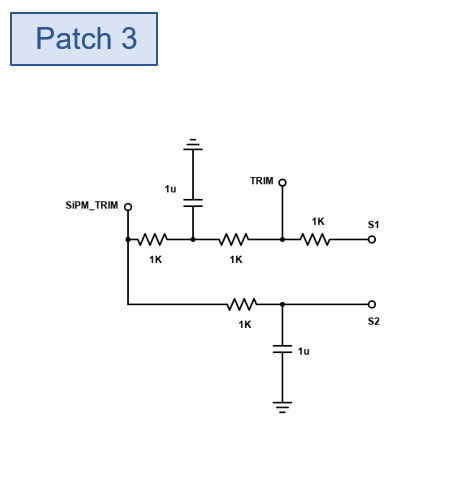
\includegraphics[width=60mm]{Images/patch_3.png}}
\subfigure[]{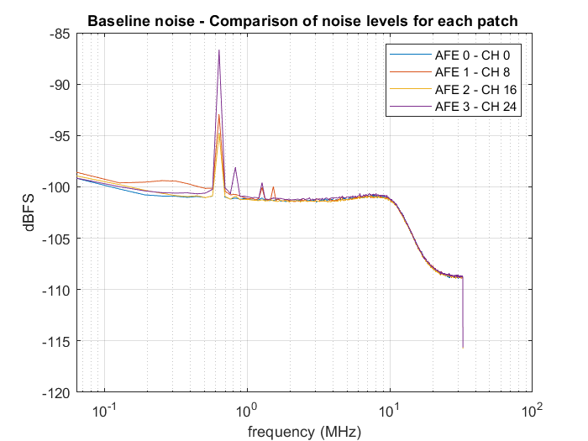
\includegraphics[width=60mm]{Images/noise_comp_patch.png}}
\caption[]{Selected filter patch at the Analog Multiplexer and TRIMM output.  a) S1 ans S2 are the analog multiplexer pins. TRIM is the BIAS TRIM voltage output. b)  Frequency spectrum  of the AFE input after the patches were applied.}
\label{fig:patches}
\end{figure}


\subsection{Cold amplifier: SNR and P.E. dynamic range}

Previous sections show test and studies performed to obtain the best SNR and dynamic range possible for DAPHNE's AFE systems. These tests were key to identify issues for both performance figures and apply modifications to the hardware in order to improve performance as was showed.

With the issues addressed, integration test of the cold and warm electronics (DAPHNE) were performed. The firsts tests were done with a very high AFE gain configuration to have a starting point to tune the systems to achieve the goals of a SNR greater than 4 and a dynamic range of 2000 P.E. The AFE gain configuration that was used for the following test was a LNA gain of $12dB$, a programmable gain amplifier PGA gain of $24dB$ and the PGA and LNA integrators ON. The cold amplifier ganging 48 SiPMs were submerged in $LN_2$, introduced into a dark box where a LED driver pulses light into the detectors via a optical fiber. The LED driver triggers with a external signal synchronized to the external trigger signal for DAPHNE.

Figure \ref{fig:fbk_hist_avg_vgain_03} show the results of the tests. The histogram in figure \ref{fig:fbk_hist_avg_vgain_03}a is produce by the integration of 40 samples after the beginning of the rising edge of the average signal. Figure \ref{fig:fbk_hist_avg_vgain_03}b shows the average single P.E. signal produced by averaging every waveform whose integral matches the second peak of the histogram. By taking the first and second peaks of the histogram, corresponding to noise and single P.E. charge respectively, the SNR figure used on-wards is defined as:

\begin{equation}
    SNR = \frac{\Delta}{\sigma_0}
\label{eq:SNR}
\end{equation}

where delta is defined as $\Delta = \mu_1 - \mu_0$ the distance between the mean values of the Gaussian fits of the peaks, shown in red, and $\sigma_0$ is the standard deviation of the fit of the peak corresponding to noise integral, the first peak. The dynamic range is defined as the peak-to-peak value of the average P.E. over the full range of the AFE ADC, in this case, $2^{14}$. 

\begin{equation}
    DR = \frac{A_{pp}}{2^{14}}
\label{eq:DR}
\end{equation}

\begin{figure}[h]
\centering
\subfigure[]{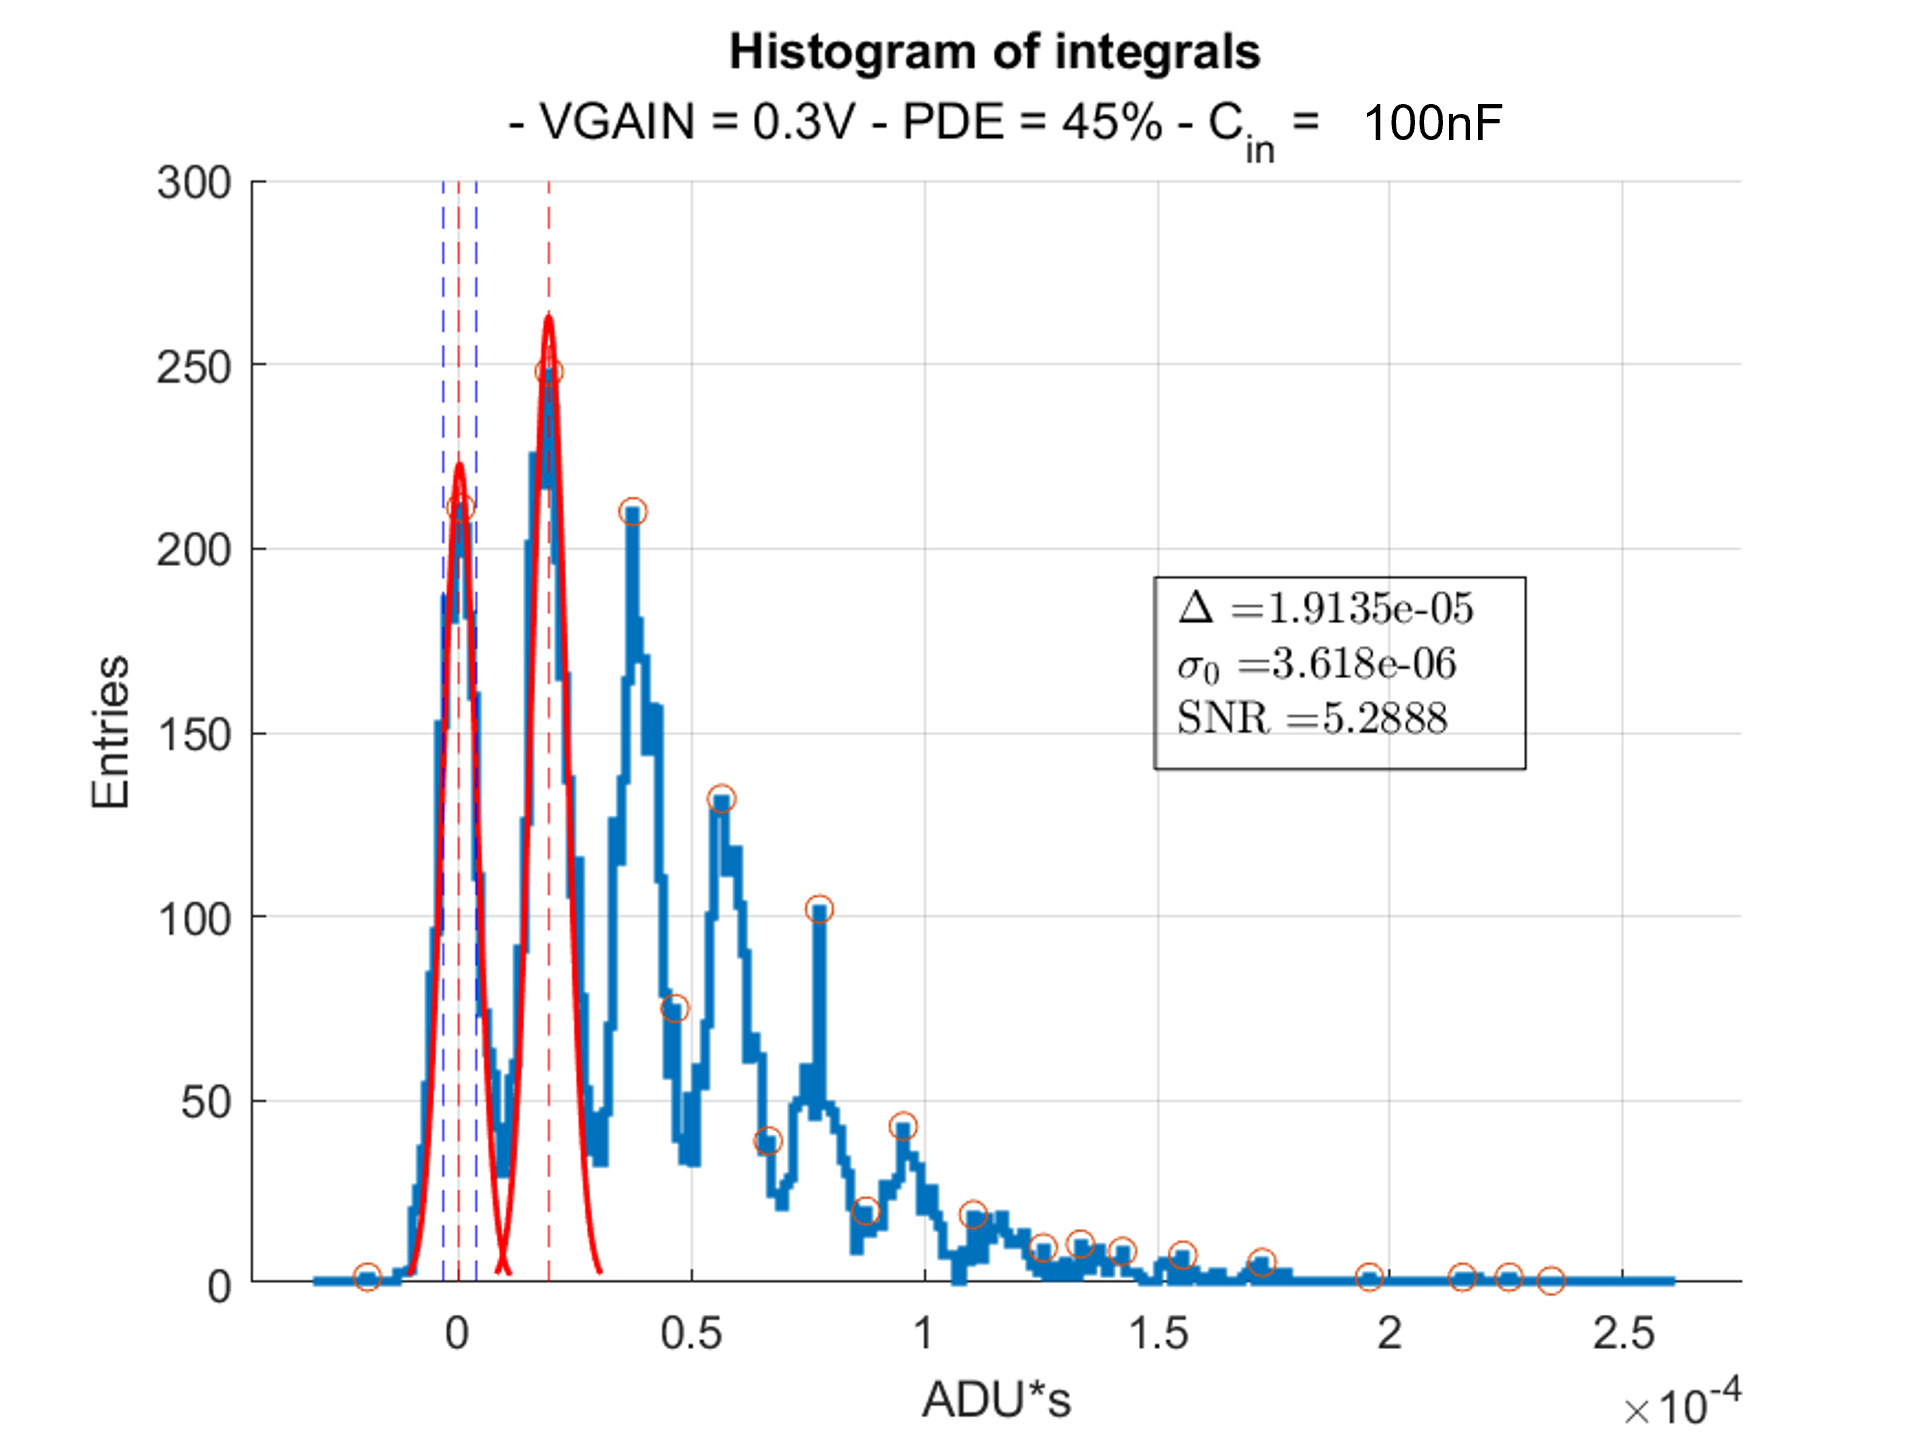
\includegraphics[width=60mm]{Images/hist_fbk_vgain_03.png}}
\subfigure[]{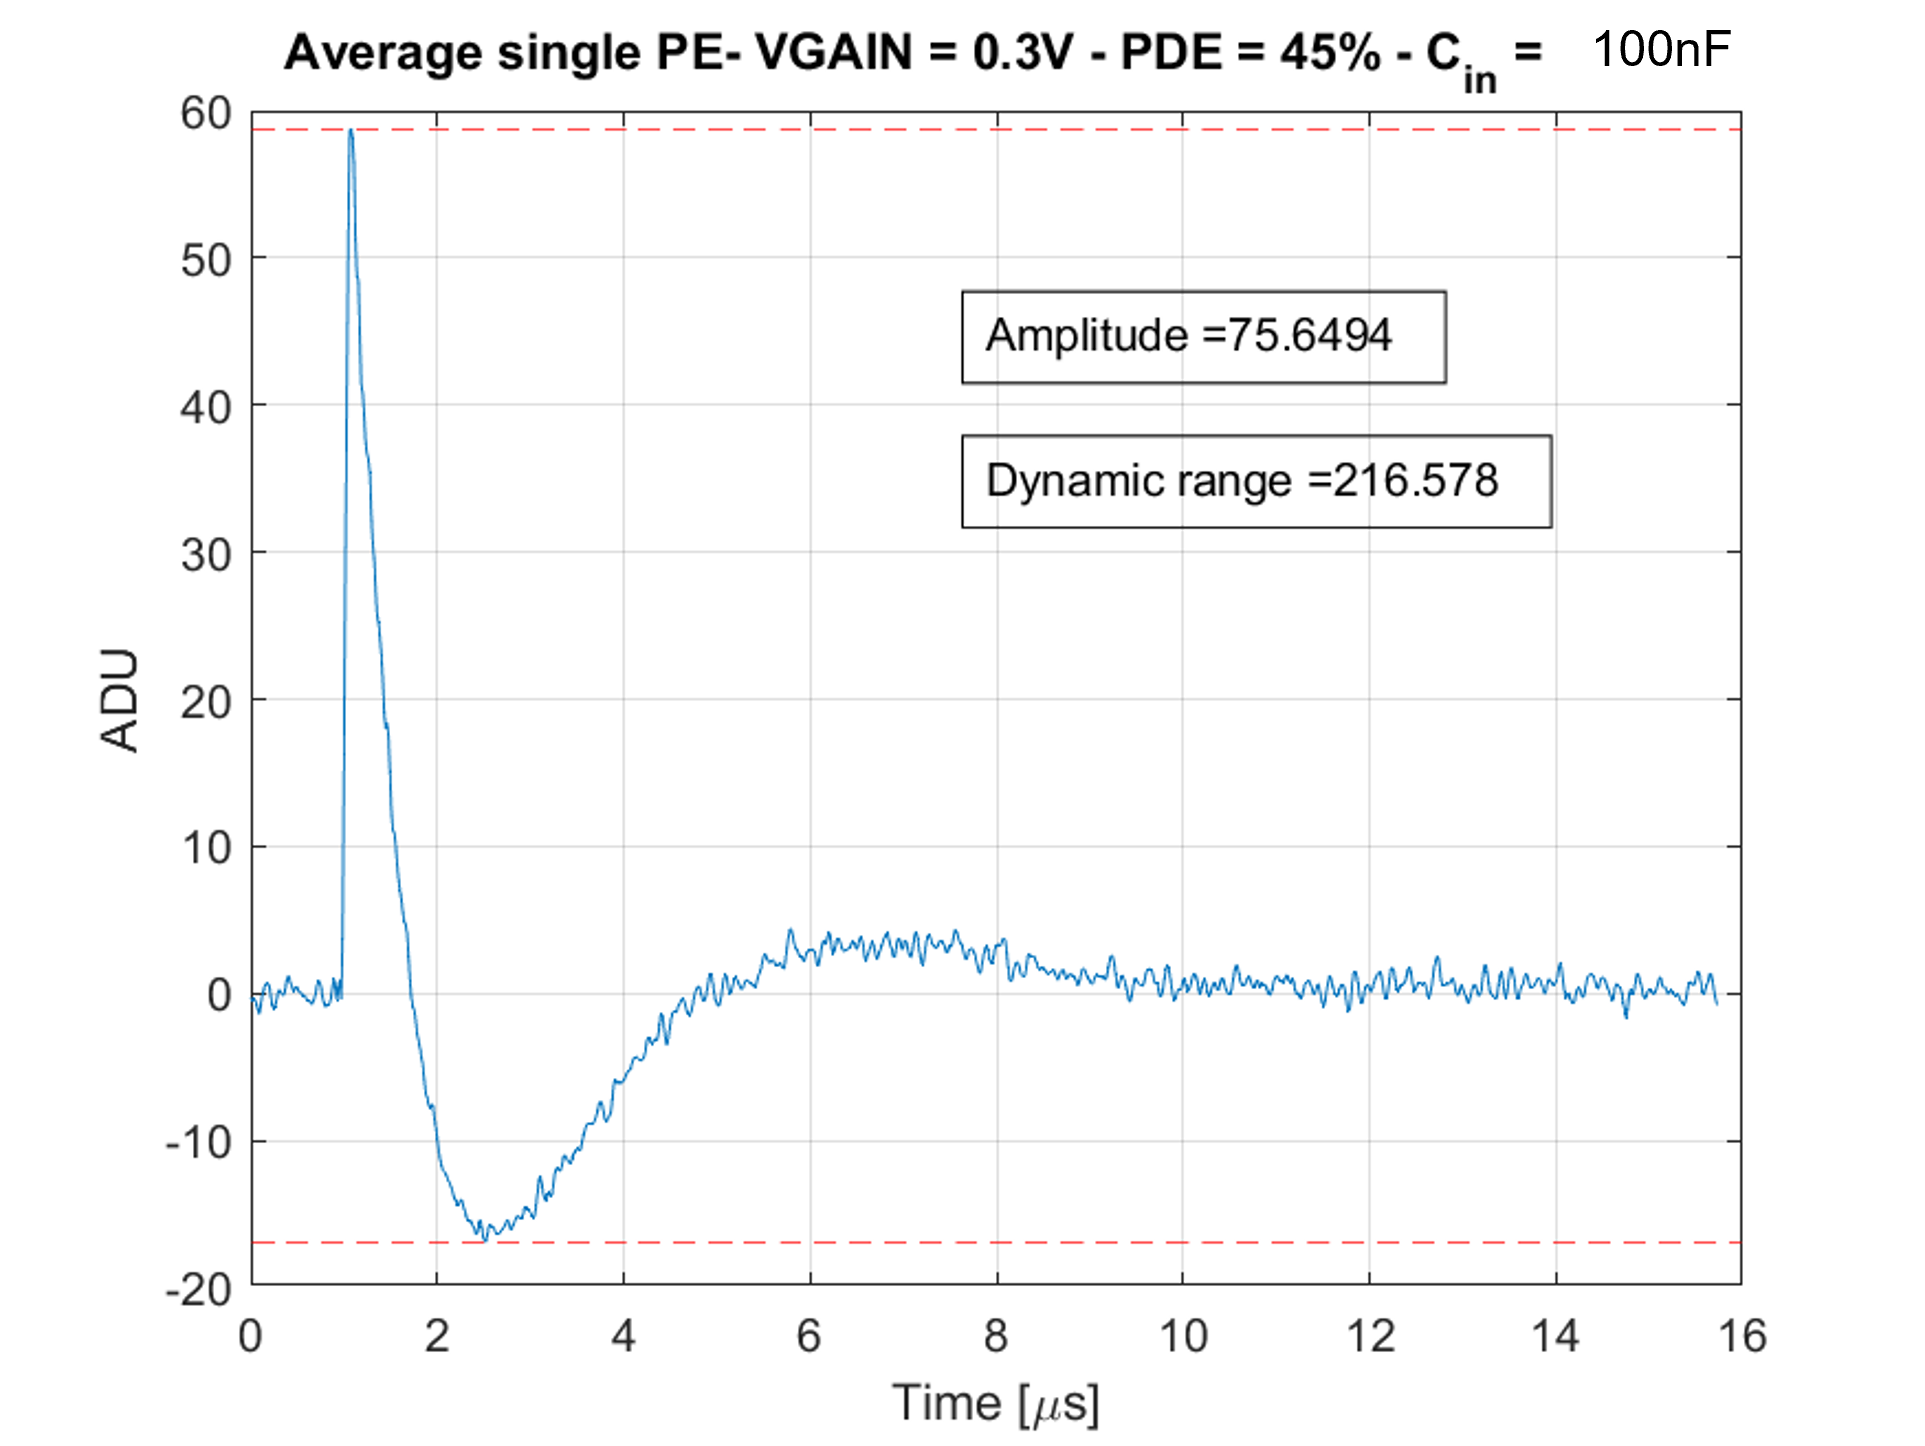
\includegraphics[width=60mm]{Images/avg_fbk_vgain_03.png}}
\caption[]{FBK-3T SiPMs cold-warm electronics integration test with VGAIN = 0.3V.  a) Histogram of charge integrals. b) Average single P.E.}
\label{fig:fbk_hist_avg_vgain_03}
\end{figure}

Applying equations \ref{eq:SNR} and \ref{eq:DR} to the data in figure \ref{fig:fbk_hist_avg_vgain_03}, a SNR of $5.29$ and a DR of $216$ P.E. is obtained. Although the SNR values comply with the requirement, the dynamic range is well below the 2000 P.E. mark. In order to calibrate the system, the following procedure was performed:

\begin{enumerate}
    \item For a given PDE configuration, in this case 45\%, and given VGAIN = 0.3V which has an overall gain of 23.4 according to the AFE5808 datasheet, the average single P.E. peak-to-peak amplitude is found by: \begin{equation}
        A_{1P.E.(0.3V)} = \frac{2^{14}}{216} = 76 ADU
    \end{equation}
    \item The target amplitude for 2000 P.E. is:
    \begin{equation}
        A_{2000P.E.} = \frac{2^{14}}{216} = 8 ADU
    \end{equation}
    \item The desired gain to obtain a single P.E. of amplitude 8 ADU is 
    \begin{equation}
        G_{1P.E.(8ADU)} = \frac{A_{2000P.E.}G_{0.3V}}{A_{1P.E.(0.3V)}} = \frac{8*23.4}{76} = 2.46(7.83)
    \end{equation}
\end{enumerate}

Taking as a reference table 16 of the AFE5808 datasheet \cite{afe5808a}, which give the overall gains values at 0.1V VGAIN intervals, a fit was performed to obtain the VGAIN value to have a gain of $7.83dB$, resulting in a VGAIN configuration of 0.86V, which gives a DR = 1919 P.E. Increasing VGAIN to $0.89V$, a DR = 2177 P.E. with a SNR = 4.34 was obtained, as can be seen in figure \ref{fig:fbk_hist_avg_vgain_2000}.

\begin{figure}[h]
\centering
\subfigure[]{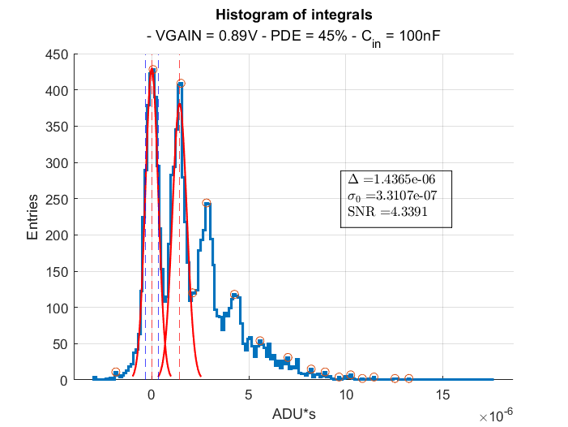
\includegraphics[width=60mm]{Images/hist_fbk_vgain_2000.png}}
\subfigure[]{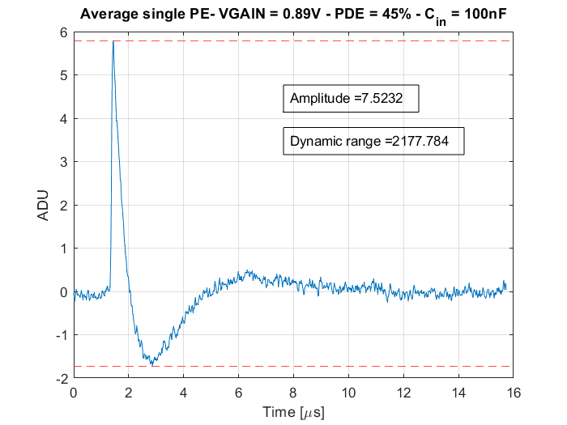
\includegraphics[width=60mm]{Images/avg_fbk_vgain_2000.png}}
\caption[]{FBK-3T SiPMs cold-warm electronics integration test with VGAIN = 0.89V.  a) Histogram of charge integrals. b) Average single P.E.}
\label{fig:fbk_hist_avg_vgain_2000}
\end{figure}

Until now, all test were performed with the AFE integrators ON. The AFE integrators are internal DC compensation that have the behavior of a high pass filter with a cut-off frequency of 80kHz. Given that the integrators act as a high pass filter, the waveforms are always centered at mid-range scale reducing the dynamic range in half and therefore, they must be disabled.

Figure \ref{fig:fbk_noise_1f}b shows a notable deterioration of the SNR figures when the LNA and PGA integrators are OFF. This main cause for this deterioration is the presence of a $1/f$ spectrum component seen in figure \ref{fig:fbk_noise_1f}a which does not allow a stable pedestal value. Also, there is the fact that the integration process is susceptible to low frequency components. 

\begin{figure}[h]
\centering
\subfigure[]{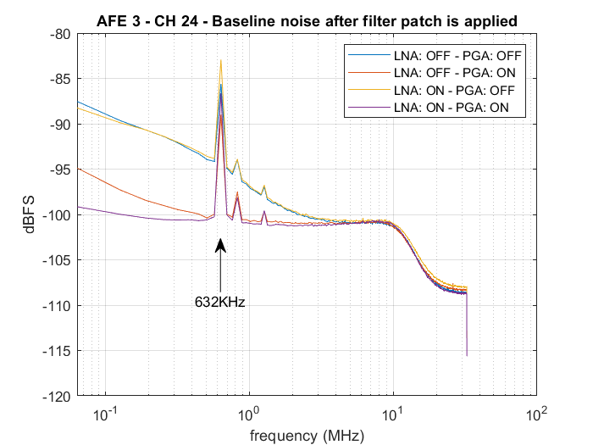
\includegraphics[width=60mm]{Images/noise_int_off_1f.png}}
\subfigure[]{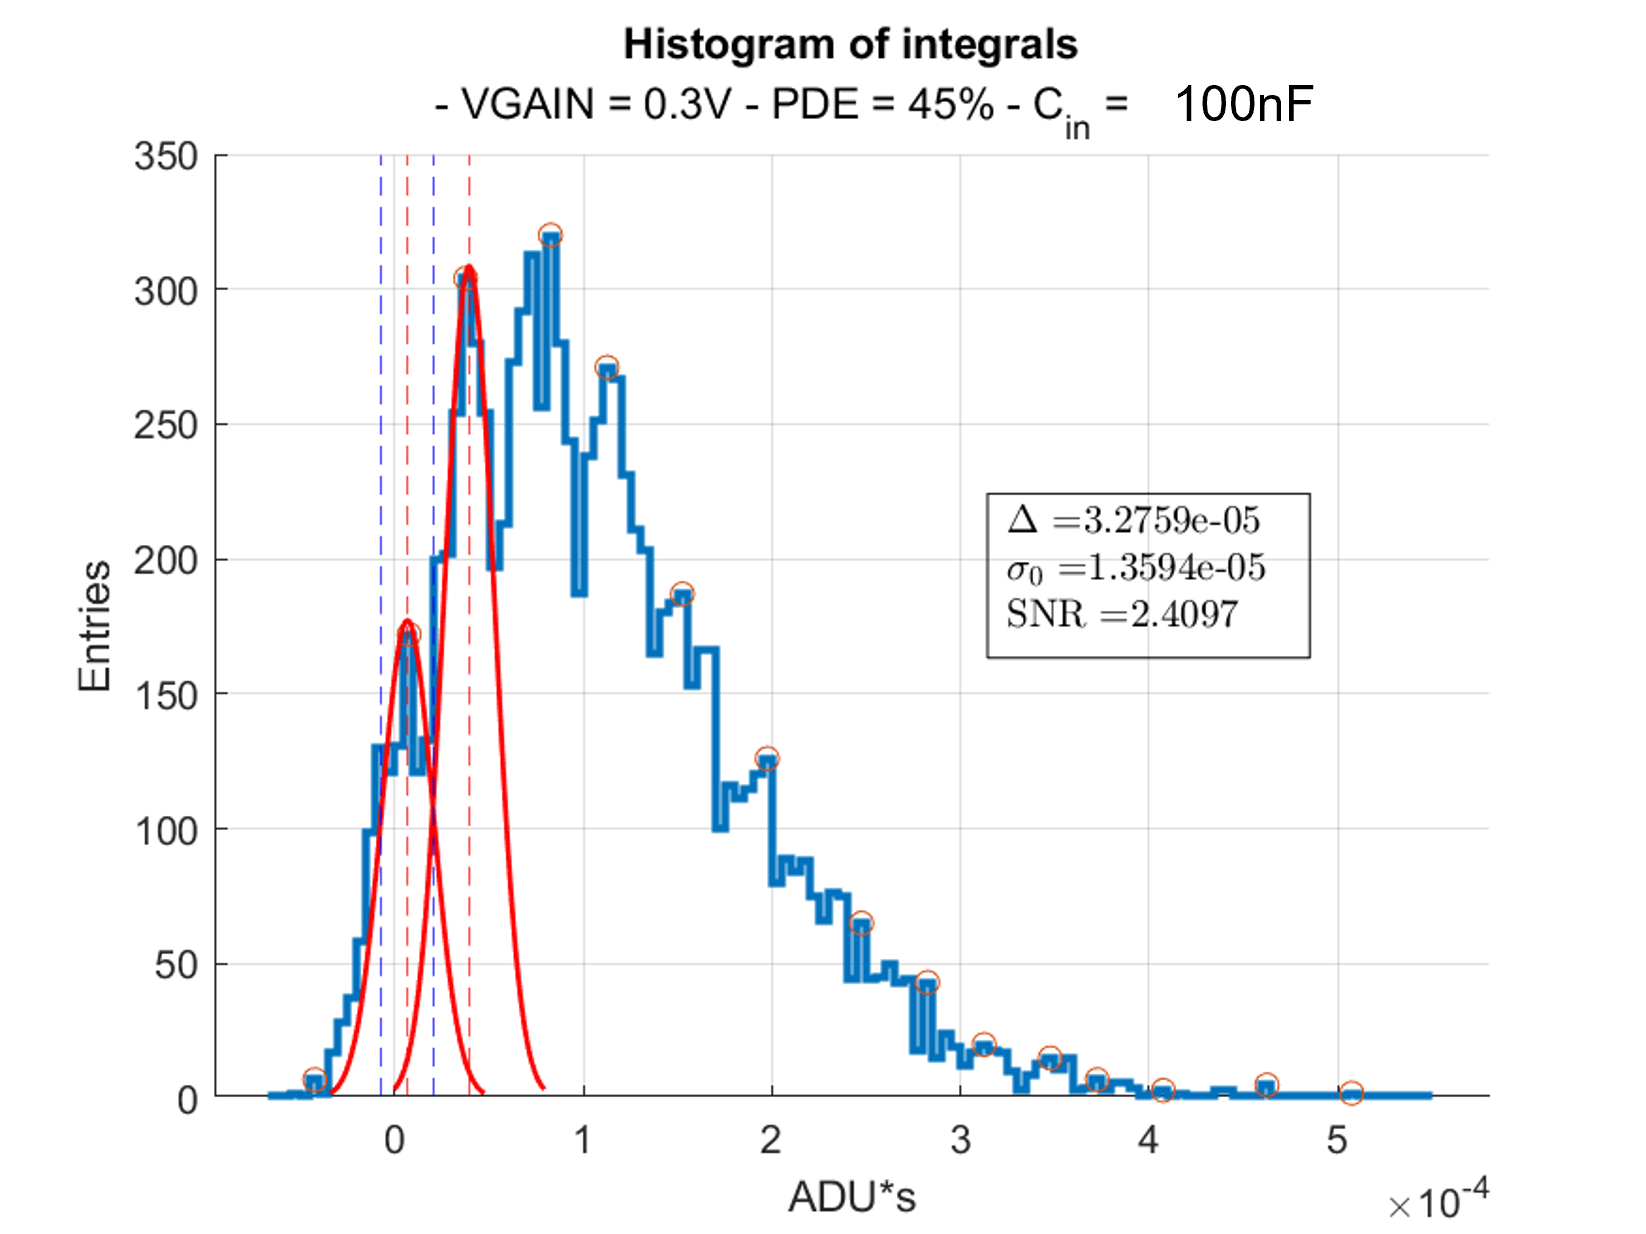
\includegraphics[width=60mm]{Images/hist_noise_int_off.png}}
\caption[]{Effect of turning OFF the AFE integrators.  a) Input frequency spectrum. b) Histogram of charge integrals for a VGAIN = 0.3V configuration.}
\label{fig:fbk_noise_1f}
\end{figure}

The proposed solution to this issue was to develop IIR digital filters inside the FPGA that emulate the response of the AFE integrators with the capability to recover the pedestal value. Figure \ref{fig:dig} shows the block design of the implemented filter inside DAPHNE's FPGA. This filter has two main modules, a low pass filter LPF and a high pass filter HPF. Data from AFE5808's ADC (X[15:0]) enters the LPF, where an average of $2^n$ samples is performed ($n$ is configurable and set to 21). The average value gets substracted from the data and the result is fed to the HPF with filter coefficients to emulate the response of the AFE integrators. Finally, the average value is added back to the filtered data to recover the pedestal. The filter hast two outputs, pedestal recovered and pedestal removed, where the latter is the waveform centered around zero.   

\begin{figure}[h]
\centering
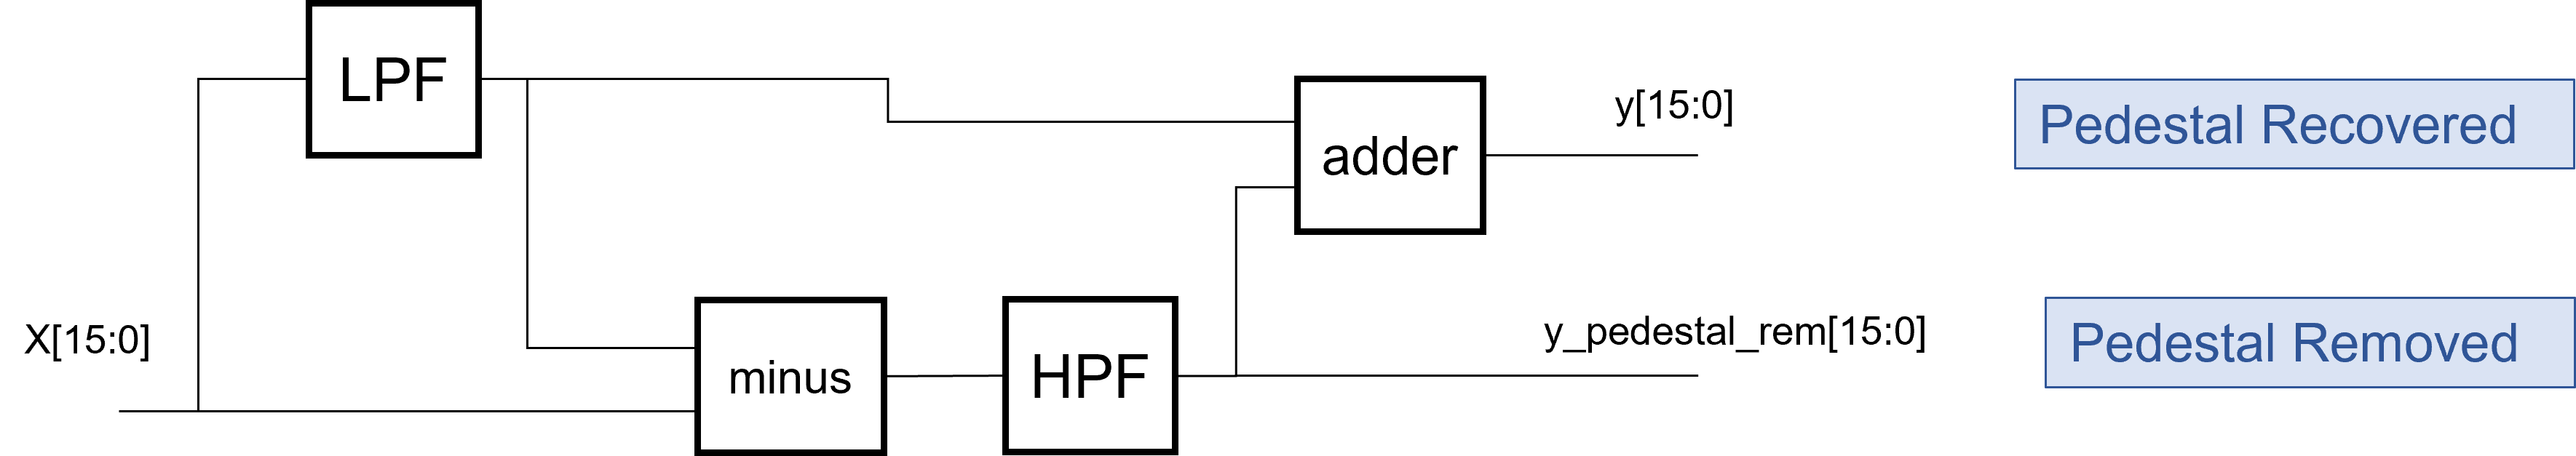
\includegraphics[width=120mm]{Images/digital_filter_1.png}
\caption[]{Digital filter implemented in the FPGA.}
\label{fig:dig}
\end{figure}

Figure \ref{fig:fbk_filtered} shows the response of the implemented filter. Although the filter behaves in the same way as the AFE integrator filters, as can be seen in figure \ref{fig:fbk_filtered}b where a comparison is made between data acquired with the AFE integrators OFF, AFE integrators ON, filtered offline and filtered online in the FPGA; the histogram in figure \ref{fig:fbk_filtered}b shows a deterioration in the SNR of around 0.5.

\begin{figure}[h]
\centering
\subfigure[]{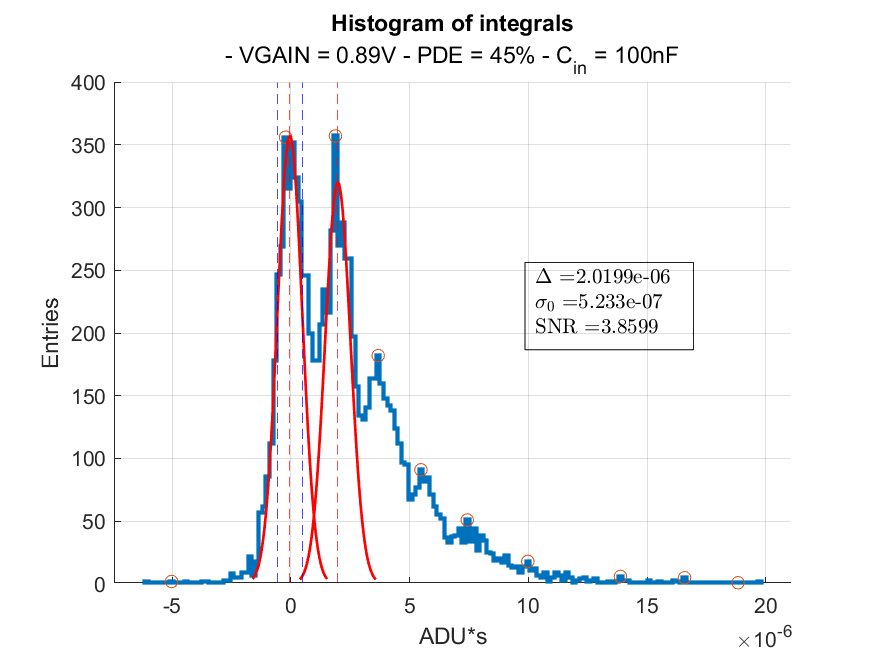
\includegraphics[width=60mm]{Images/hist_fbk_filtered.png}}
\subfigure[]{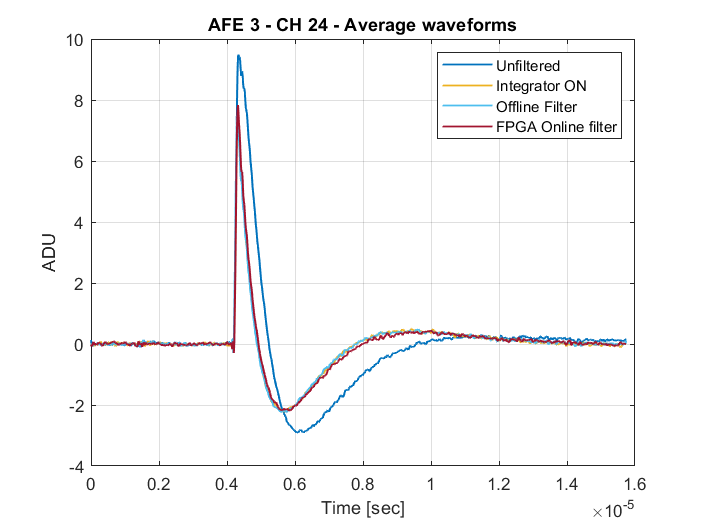
\includegraphics[width=60mm]{Images/avg_filtered.png}}
\caption[]{FBK-3T SiPMs implemented filter response.  a) Histogram of charge integrals. b) Average single P.E.}
\label{fig:fbk_filtered}
\end{figure}

\subsection{DAPHNE triggering capabilities}

To test DAPHNE triggering capabilities, the cold amplifier was connected to a X-ARAPUCA supercell ganging 48 Hamamatsu SiPMs submerged in $LN_2$. In the same manner as the FBK SIPMs, the Hamamatsu SiPMs were illuminated with the LED driver via an optical fiber, to acquire data with the external trigger and the implemented internal self-trigger. 

First, in order to have raw data, waveforms were acquired using the external trigger with the AFE integrators OFF. The acquired data was also used to confirm that Hamamatsu SiPMs behave similarly to FBK-3T producing SNR and DR values in the same order. Figure \ref{fig:hpk_hist_avg} shows that a $SNR = 4.5$ and a $DR = 2003$ is obtained with a configuration of $PDE = 45\%$ and $VGAIN = 0.89V$. In figure \ref{fig:hpk_filt_comp}, a comparison between the implemented FPGA filter and the AFE integrators is presented at a $PDE = 50\%$. This comparison is made at a $PDE = 50\%$ instead of $45\%$ to have a better resolution, since the peaks are more defined with larger overvoltage values. The result is consistant with FBK measurements, the implemented FPGA filter has a reduced SNR value of around 0.5 compared with the AFE integrator filters and should expect that at $PDE = 45\%$, the SNR value is around 4.   

Until now, waveforms were acquired using the external trigger signal synchronized with the LED driver. In order to have self-trigger capabilities, i.e. that DAPHNE acquires waveforms at a configured P.E. level using as a reference the streaming ADC data, a trigger processor module has to be implemented inside the FPGA that asserts the trigger flag at the correct P.E. level. The fist versions of such module was implemented, simulated and tested. 

\begin{figure}[h]
\centering
\subfigure[]{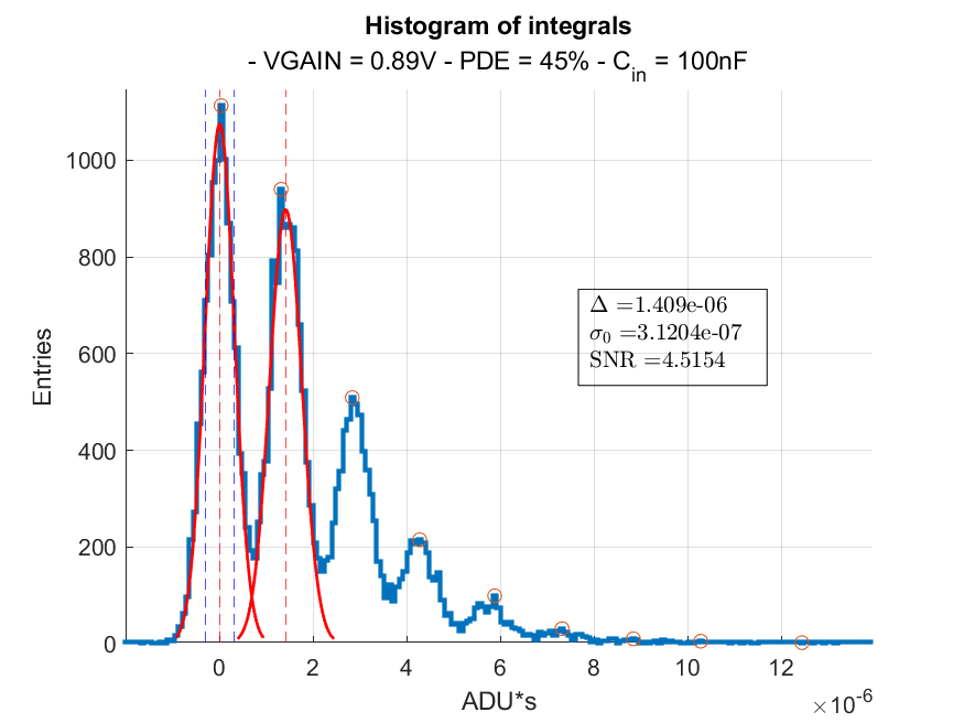
\includegraphics[width=60mm]{Images/hpk_hist_45.png}}
\subfigure[]{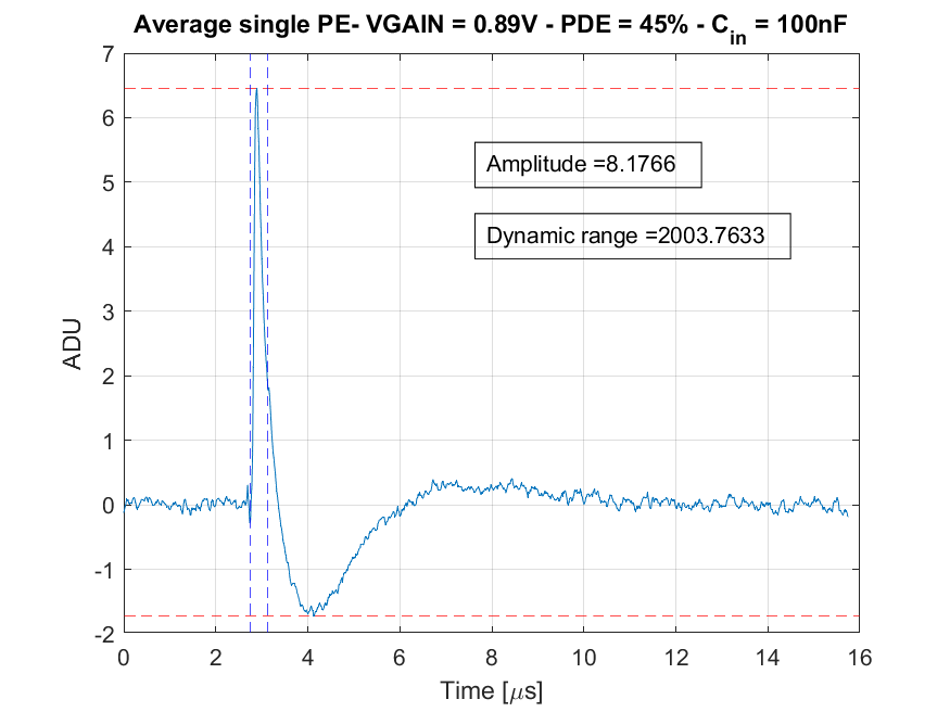
\includegraphics[width=60mm]{Images/hpk_avg_45.png}}
\caption[]{Hamamatsu SiPMs integration test with VGAIN = 0.89V and 45\% PDE.  a) Histogram of charge integrals. b) Average single P.E.}
\label{fig:hpk_hist_avg}
\end{figure}

\begin{figure}[h]
\centering
\subfigure[]{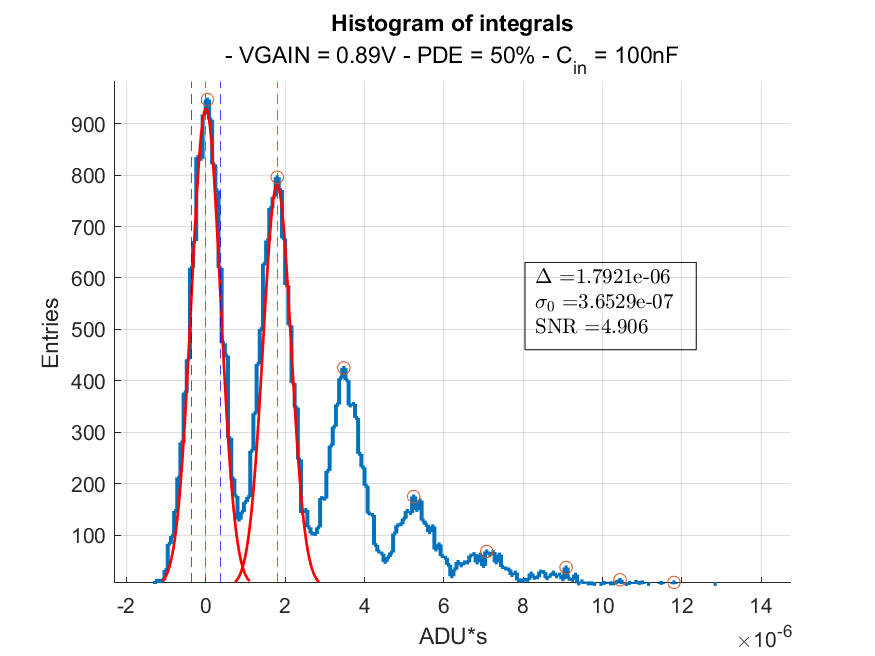
\includegraphics[width=60mm]{Images/hpk_hist_50_filtered.png}}
\subfigure[]{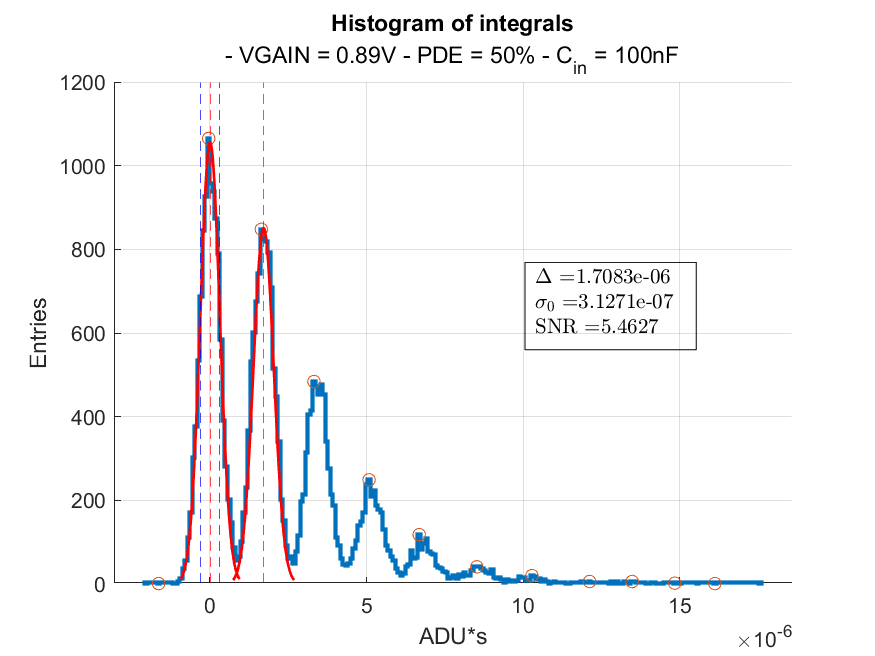
\includegraphics[width=60mm]{Images/hpk_hist_50.png}}
\caption[]{Hamamatsu SiPMs implemented filter response.  a) Histogram of charge integrals - FPGA filtered. b) Histogram of charge integrals - AFE integrators ON.}
\label{fig:hpk_filt_comp}
\end{figure}

Figure \ref{fig:trigger_processor} shows the schematic for the implemented trigger processor. It consist of three main modules: an integrator filter that approximates the behavior of a moving average filter; a threshold detector that assert a signal when the filtered data goes beyond a configured value; and a zero crossing detector module that performs a constant fraction discriminator and asserts a signal when the zero-crossing is detected. 

\begin{figure}[h]
\centering

\includegraphics[width=120mm]{Images/trigger_processor.png}
\caption[]{Scheme of the trigger processor implemented in DAPHNE's FPGA.}
\label{fig:trigger_processor}
\end{figure}

The coincidence of the assertion flags signals a trigger condition that is fed to the external modules that handle the storage of the acquired data. The integrator filter is implemented using the same architecture as the HPF in figure \ref{fig:dig}, using different coefficients. The input of the module is the "pedestal removed" signal from the FPGA digital filter. The integrator filter approximates the response of a moving average filter of 25 samples, just as the integration window shown in figure \ref{fig:filter_figures}a. The peak value of the filtered waveform is equal to the integration process, as can be noted by the red dashed lines. Figure \ref{fig:filter_figures}c shows the histogram of the peak values where the obtained SNR value is around 4.15.

The output of the integrator filter is fed to the threshold detector module and the zero crossing detector module. The threshold detector module is very straightforward, it asserts the threshold flag when the input value is greater than the configured threshold value. The threshold value can be tuned using the histogram shown in figure \ref{fig:filter_figures}c. The mean values of the fitted Gaussian peaks can be considered as the $n$ P.E. value and the intersection of the curves can be considered $n + 1/2$ P.E.  

The zero crossing module deals with the known problem of amplitude walk. If a simple threshold flag is used for triggering, the asserted signal will have a time jitter caused by the fact that the integrated signal has the same rise time always, and is independent of the amplitude, hence small P.E. signals will take longer to reach the threshold value than larger P.E. signals. The module takes the input signal, inverts and delays it; and then performs the subtraction from the original signal, creating a bipolar signal. The zero crossing time of the bipolar signal is time independent of the amplitude. Figure \ref{fig:filter_figures}b show the described process for a delay of 40 samples. Later studies showed that keeping the delay value below the distance between 10\% to 90\% yields the best results minimizing the jitter. The jitter studies are not included in this report but will be presented later on. 


\begin{figure}[h]
\centering
\subfigure[]{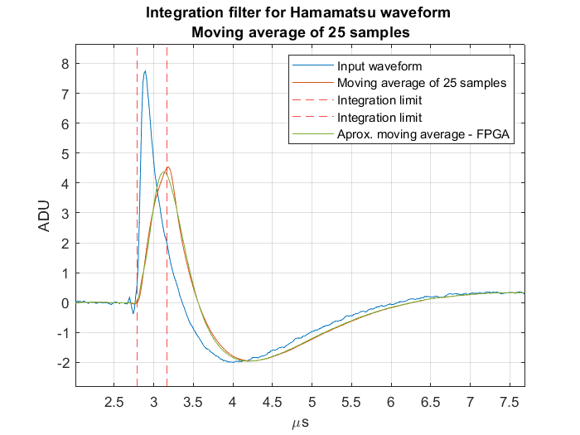
\includegraphics[width=60mm]{Images/avg_movmean.png}}
\subfigure[]{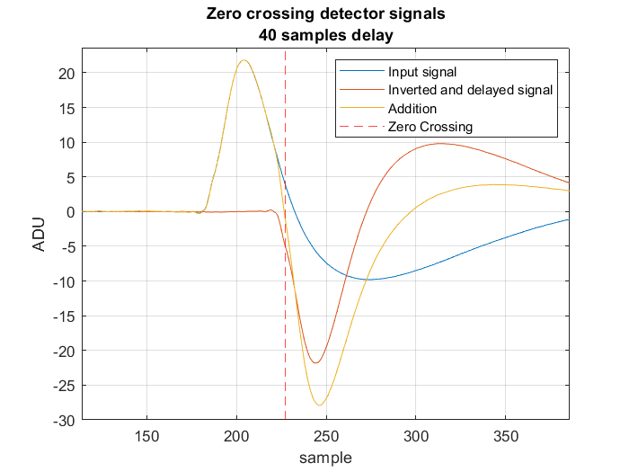
\includegraphics[width=60mm]{Images/zero_crossing.png}}
\subfigure[]{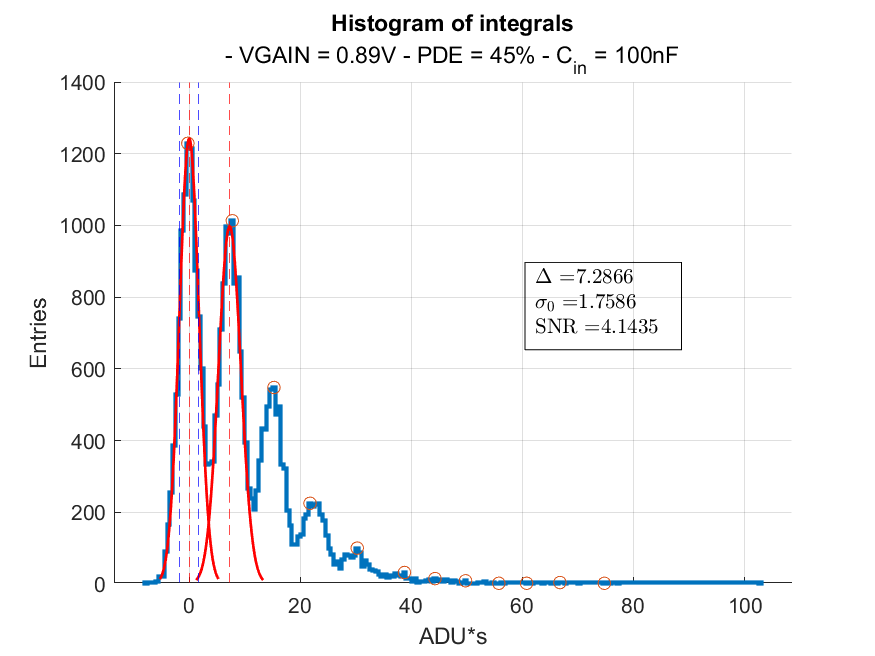
\includegraphics[width=60mm]{Images/histogram_movmean_avg.png}}
\subfigure[]{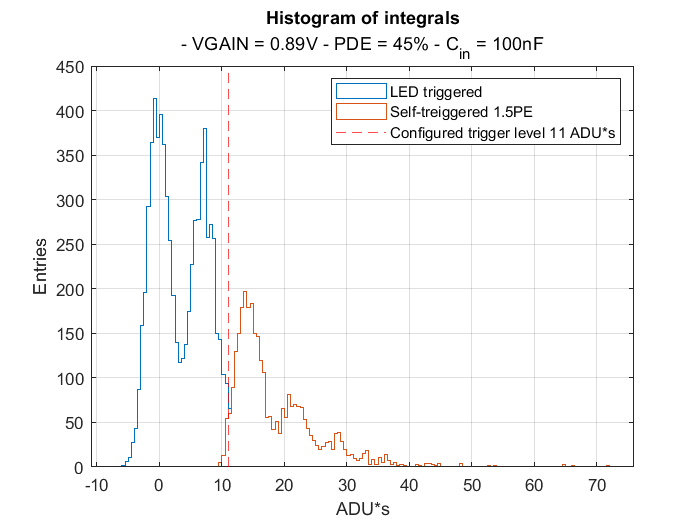
\includegraphics[width=60mm]{Images/hpk_level_11_1_5PE.png}}
\caption[]{Trigger processor integration process. a) Average input waveform and a comparison of the result of the integrator filter and a classic moving average filter. b) Zero crossing detector process. c) Histogram of charge integrals - Peak value of the integrator filter. d) Hardware behavioral simulation - Peak values of the triggered signals.}
\label{fig:filter_figures}
\end{figure}

To test the trigger processor module, a behavioral simulation of the implemented hardware was performed in Iverilog using the raw unfiltered data. The simulation takes the raw unfiltered data and outputs the trigger flag as a boolean vector. In this way, it is know at what point exactly the trigger was asserted compared to the LED reference. Also, it is possible to obtain the intermediate waveforms, such as the output waveform of the integrator module inside the trigger processor and elaborate the histogram shown in blue in figure \ref{fig:filter_figures}d. Then, taking the values that asserted the trigger, the histogram in red is elaborated and is clearly visible that the module triggered at the desired location, calibrated at 11 $ADUs$, corresponding to 1.5 P.E.  

\begin{figure}[h]
\centering
\subfigure[]{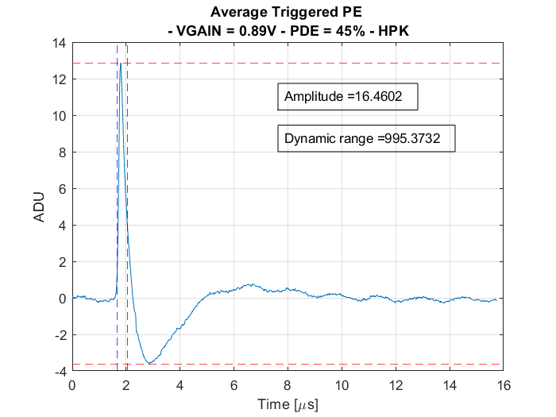
\includegraphics[width=60mm]{Images/avg_self_trigger.png}}
\subfigure[]{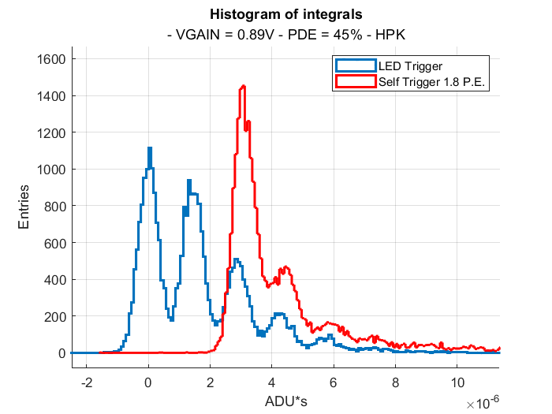
\includegraphics[width=60mm]{Images/self_trigger_comp.png}}
\caption[]{Self-trigger test with Hamamatsu supercell. a) Average waveform of the first self-triggered integral peak. b) Histograms of charge integrals}
\label{fig:self_trigger_test}
\end{figure}

The test of the self-trigger module with the cold amplifier was performed with the Hamamatsu supercell at $45\%$ PDE. Due to an error loading the incorrect firmware, the trigger was set to 1.8 P.E., calibration of 1.5 P.E. intended for a $50\%$ PDE. Nevertheless, the module behaved as expected. Figure \ref{fig:self_trigger_test} show the results of the test, were a dynamic range of 995 was obtained using the average signal of the first peak of the histogram shown in red in figure \ref{fig:self_trigger_test}b.

According to the simulations, the cut at 1.8 P.E. in the red histogram should be more pronounced, but obtaining a good precise histogram is difficult due to the jitter introduced by the self-trigger, that according to the simulation is around 10 samples.

\label{sec:testing}